% -*- TeX -*- -*- LaTeX -*-
% Standalone TikZ diagram of Monad DB architecture
\documentclass[tikz,border=5pt]{standalone}
\usetikzlibrary{positioning,shapes,arrows.meta}
\begin{document}
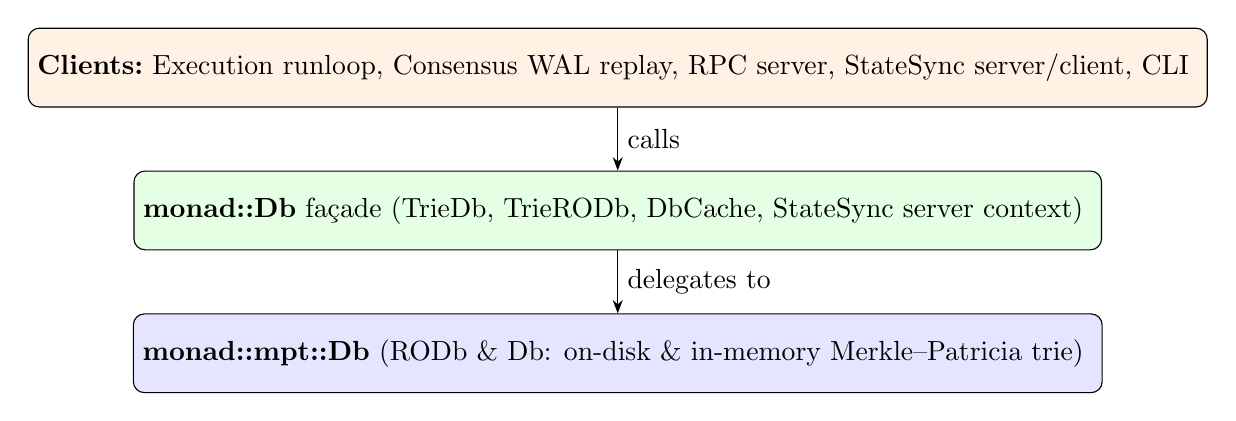
\begin{tikzpicture}[
  node distance=8mm and 12mm,
  box/.style={draw, rectangle, rounded corners, minimum width=8cm, minimum height=1cm, align=center, fill=#1!10},
  >=Stealth
]

% Raw MPT engine layer
\node[box=blue] (mpt) {
  \textbf{monad::mpt::Db}\
  (RODb \& Db: on‑disk \& in‑memory Merkle–Patricia trie)
};

% High‑level façade layer
\node[box=green, above=of mpt] (facade) {
  \textbf{monad::Db} façade\
  (TrieDb, TrieRODb, DbCache, StateSync server context)
};

% Clients layer
\node[box=orange, above=of facade] (clients) {
  \textbf{Clients:}\
  Execution runloop, Consensus WAL replay, RPC server, StateSync server/client, CLI
};

% Arrows between layers
\draw[->] (clients) -- (facade) node[midway, right] {calls};
\draw[->] (facade) -- (mpt) node[midway, right] {delegates to};

\end{tikzpicture}
\end{document}